
\documentclass[12pt,a4paper]{report}
\usepackage[utf8]{inputenc}
\usepackage{amsmath}
\usepackage{amsfonts}
\usepackage{amssymb}
\usepackage{graphicx}
\usepackage{listings}
\usepackage{fancyhdr}
\usepackage{parskip}
\usepackage{rotating}
\pagestyle{fancy}
\chead{2.1.10 - sw608f14 - Daniel S. F., Lars A, Mathias W. P. \& Søren S. A.}

\lstset{mathescape = true}
\usepackage{amsthm}
\begin{document}
\section*{Selfstudy 3}
\section*{1.}
This exercise has been answered in the last selfstudy.
\section*{26-1 Escape Problem}
\subsection*{b}
Part a greatly hints how to model a flow network.
Here is an example of a grid's (3x3) corresponding flow network, figure \ref{diagram}, where (1,1) and (2,2) are marked, with the answer to part one this can then be made into a regular flow network.

\begin{figure}
     \centering
     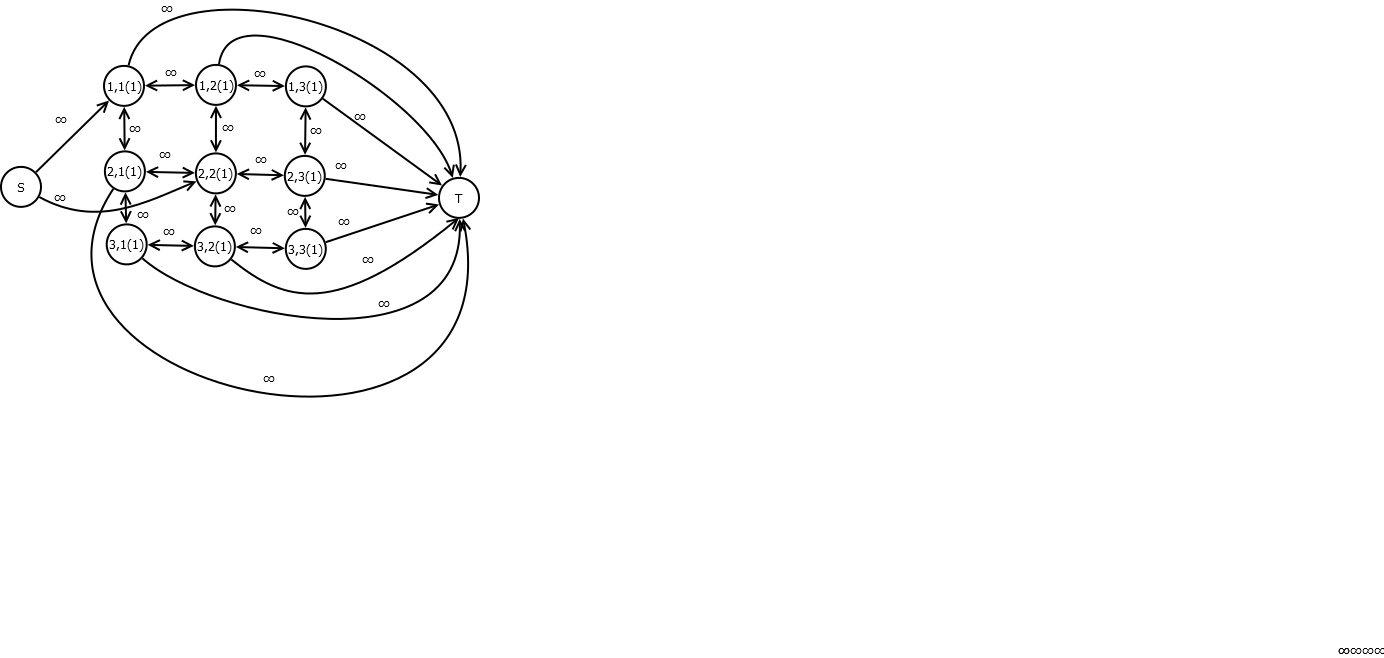
\includegraphics[scale=0.5]{diagram}
     \caption{Diagram of flow network. for exercise 26-1 b.}     
     \label{diagram}
     
\end{figure}

How the flow network will be constructed is as follows.
We very much follow figure 26.8
One source node S and a target node T is added.
Furthermore there is an edge for each field in the grid, named $v_{i,j}$. 
Each $v_{i,j}$ has weights 1 (which can afterwards be transformed into a regular flow network), and is connected to its adjacent vertices in both directions with flow 1.
S gets assigned an edge of flow $\infty$ to each start node.
Furthermore from each vertice $v_{i,j}$ where it is a border vertice, it will have an edge going from it to T with $\infty$ flow.
Then when the network has been converted to a flow network, it is just a matter of running Edmond Karp from S to T and see whether the flow reaching T is lesser or greater than $m$.
Its running time is then $O(V^2E$) as constructing the network could be done in linear time.

\section*{17-2}
\subsection*{a.}
For search, the problem will consist of searching in the arrays $A_i$ where $n_i = 1$.
A search that can be used is binary search.
Here is an analysis of its worst case running time.
$$\sum\limits_{i=0}^{k-1} lg(2^i) = \sum\limits_{i=0}^{k-1} i = \frac{1}{2} * (k-1) * k = O(k^2) = O(lg^2(n+1)) = O(lg^2(n))$$

\subsection*{b.}
To get a first understanding of how the insertion would work, here is a sketch where 1 means the array is full and 0 means it is empty.
9 insertions will then look like this in respect to which arrays are full.

\begin{tabular}{|c|}
\hline 
0000 \\ 
\hline 
1000 \\ 
\hline 
0100 \\ 
\hline 
1100 \\ 
\hline 
0010 \\ 
\hline 
1010 \\ 
\hline 
0110 \\ 
\hline 
1110 \\ 
\hline 
0001 \\ 
\hline 
1001 \\ 
\hline 
\end{tabular}

From the example, it can be seen that when you INSERT, you go through your arrays $A_0 ... A_{k-1}$ until you find an array that is empty. If $A_j$ is the first array found empty, all the previous arrays $A_0 ... A_{j-1}$ will then be emptied and inserted into $A_j$, in addition to the new element to be inserted, in sorted order. The reason for this is that $A_j$ can contain all the previous arrays plus an additional element. To care of the insertion in sorted order of the previous arrays is not a problem as those arrays are already sorted, and a technique similar to mergesort can then be used.

The worst case example is if all the arrays $A_0 .. A_{k-1}$ are full. And you then have to insert a new element.
We use the advantage that all the previous arrays are already sorted, so the cost will be that of merging the arrays which will be $2^0 + 2^1 + 2^2 ... 2^{lg(n)} = O(n)$.

For amortized cost, if you think about it, when you insert an element you can pay $lg(n)$\$ as that is the maximum times the element can be moved for future insertions. The amortized cost for an insertion is then $O(lg(n))$ and is cheaper than the worst case cost that was $O(n)$.

\subsection*{c.}
If we have 9 deletions where at start the first 4 arrays are full it would like this this:

\begin{tabular}{|c|}
\hline 
1111 \\ 
\hline 
0111 \\ 
\hline 
1011 \\ 
\hline 
0011 \\ 
\hline 
1101 \\ 
\hline 
0101 \\ 
\hline 
1001 \\ 
\hline 
0001 \\ 
\hline 
1110 \\ 
\hline 
0110 \\ 
\hline 
\end{tabular} 

So how the deletion would be a reverse insertion, regarding how the arrays should be filled. Which would be an unmerging basically.
For that reason the cost of deletion would be $O(n)$
\end{document}